\documentclass[]{report}

% All Dependencies

\usepackage{graphicx}
\usepackage{float}
\usepackage{amsmath}
\usepackage{amsfonts}
\usepackage{wasysym}


% Title Page
\title{MATH 4820 - Homework 8}
\author{Jack Reilly Goldrick}


\begin{document}
	\maketitle
	
	
	\section{Problem 1:  Exercise 6.5.2}
	
	
	\begin{itemize}
		\item The obvious solution $y_0 = \sqrt[3]{2}$
		
			\subitem{i. } Using the Roots of Unity  n = 3 we have:
				
				\subsubitem{1. }  $\omega_{1} = e^{\frac{2 \pi}{3} i} $
				

				
				\subsubitem{2. }  $\omega_{2} = e^{\frac{4 \pi}{3} i} $
				
			\begin{itemize}
				\item This gives us another solution $y_2  = \omega_{1} y_0 = \sqrt[3]{2} e^{\frac{2 \pi}{3} i}$
				
				\item Using the Final Root of Unity we have:  $y_3  = \omega_{2} y_0 = \sqrt[3]{2} e^{\frac{4 \pi}{3} i}$
			\end{itemize}
			
	\end{itemize}
	
	
	
	
	\section{Problem 2}
	
	
	\begin{itemize}
		\item Since this Cubic is depressed, we can already identify $p$ and $q$:
		
		$$ p = 15 \land q = 4 $$
		
		
		\item Using Cardono's Formula we have:
		
		$$ u = \sqrt[3]{2 + 11i} = 2 + i$$
		
		$$ v = \sqrt[3]{2 - 11i} = 2 - i$$
		
		
		
		\item Thus the solution that is $x = 2$ is
		
		$$ x = \sqrt{y} = \sqrt{u + v } = \sqrt{4} = 2$$
		
		\item using the roots of unity for n = 3 we have:
		
		\begin{itemize}
			\item $\omega_{1} = e^{\frac{2 \pi}{3} i} $
			
			\item $\omega_{2} = e^{\frac{4 \pi}{3} i} $
		\end{itemize}
		
		
		
		\begin{itemize}
			\item Permuting the solution $x$ with the first and second root we have 
			
			$$y_2 = \omega_{1} u + \omega_{2} v = -2 - \sqrt{3}$$
			
			$$y_3 = \omega_{2} u + \omega_{1} v =  \sqrt{3} - 2$$
		\end{itemize}
		
	\end{itemize}
			





\section{Problem 3}
\begin{figure}[H]
	\centering
	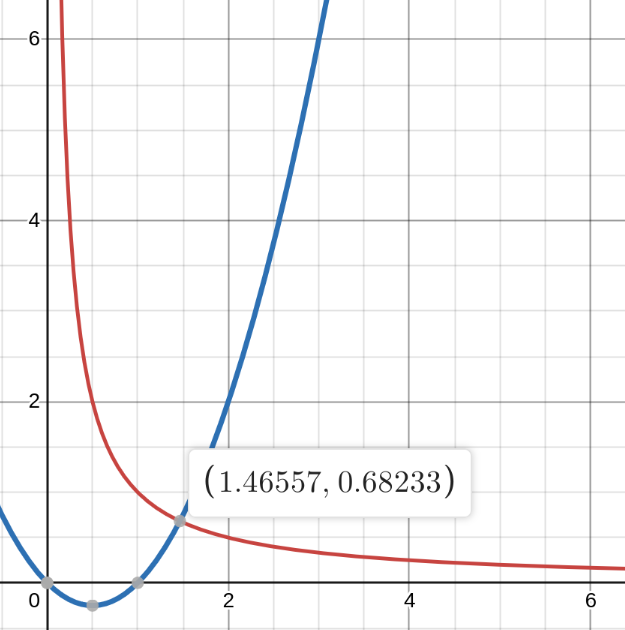
\includegraphics[width=0.7\linewidth]{pics/3}
	\caption{}
	\label{fig:3}
\end{figure}


\begin{itemize}
	\item Equating the two continuous relations we have the following polynomial of x:
	
	$$ 0 = x^3 - x^2 - 1$$
	
	
	\item Depressing the cubic with the substitution $x = t + \frac{1}{3}$ we have:
	
	$$ 0 = t^3 - \frac{1}{3} t - \frac{29}{27}$$
	
	
	\item Using Cardano's formula for $p = \frac{1}{3} \land q = \frac{29}{27}$ we have:
	
	
	$$ u = 2^{\frac{2}{3}} \frac{\sqrt[3]{3 \sqrt{93} +29}}{6}$$
	
	$$ v = 2^{\frac{2}{3}} \frac{\sqrt[3]{29 - 3 \sqrt{93}}}{6}$$
	
	\item Thus the desired real solution is $ x = u + v + \frac{1}{3} = 1.1322378985432 + \frac{1}{3} = 1.46557123188$ Which is consistent with the graph above.
	
\end{itemize}


	\begin{flushright}
		\smiley{}
	\end{flushright}
	
	
\end{document}          
